\section{Background and Related Work}
In this section, we present the necessary background knowledge about weights pruning and low-rank factorization. Note that we only focus on unstructured weights pruning since structured pruning is model architecture-dependent.
\subsection{Weights Pruning}
\label{sec:pruning}
We first establish some shared notations for different weights pruning algorithms. 
Let $\bm{W}\in \mathbb{R}^{n\times m}$ denote a generic weight matrix in a PLM. In order to determine which elements in $\bm{W}$ are pruned, an importance score matrix $\bm{S}\in \mathbb{R}^{n\times m}$ is correspondingly introduced. The smaller $S_{i,j}$ is, the larger the probability of $W_{i,j}$ will be pruned. Given the importance scores, a pruning strategy $f_{prune}(\cdot)$ computes a binary mask matrix $\bm{M}\in \{0,1\}^{n\times m}=f_{prune}(\bm{S})$, 
and the forward process for an input $x$ becomes $y=(\bm{W}\odot\bm{M})x$, 
where $\odot$ denotes element-wise multiplication.

\paragraph{Zero-order Weights Pruning} Zero-order weights pruning refers to the family of algorithms that only use the value of weight as importance measure.
For example, magnitude-based weights pruning~\cite{mag,chen2020lottery} adopts the absolute weight value as importance score, i.e., 
$\bm{S}_{i, j}=|\bm{W}_{i, j}|$. The typical choice of $f_{prune}(\cdot)$ is to remove $v\%$ percent of weights with the smallest importance:
\begin{align}
	\bm{M}_{i,j}=
	\begin{cases} 
		0, & \text{if }\bm{S}_{i,j}~\text{is the smallest }v\%\\
		1,  & \text{otherwise}  
	\end{cases}
	\label{eq:zero}
\end{align}
Different sparsity can be obtained by varying $v$.

\paragraph{First-order Weights Pruning} Unlike zero-order weights pruning where $\bm{S}$ is directly derived from $\bm{W}$, first-order methods treat 
$\bm{S}$ as learnable parameters and jointly train it with model weights 
during fine-tuning. For example, SMvP~\cite{movement} and CAP~\cite{cap}
implements $f_{prune}(\cdot)$ using a global threshold $\tau$:
\begin{align}
	\bm{M}_{i,j}=
	\begin{cases} 
		0, & \text{if }\bm{S}_{i,j}\le \tau\\
		1,  & \text{otherwise}  
	\end{cases}
	\label{eq:first}
\end{align}
Since the gradient of the thresholding function is 0 everywhere, straight-through estimator~\cite{st} is used as an approximation. The importance score $\bm{S}_{i,j}$ of $\bm{W}_{i,j}$ up to training step $T$ can be expressed as $\bm{S}_{i,j}=-\sum_{t\le T}(\frac{\partial \mathcal{L}}{\partial \bm{W}_{i,j}})^{(t)} \bm{W}_{i,j}^{(t)}$, where $\mathcal{L}$ is the loss function.
In this setting, different sparsity can be obtained by varying $\tau$.


\subsection{Low-rank Factorization}
\label{sec:lr}
Given the weight matrix $\bm{W}\in \mathbb{R}^{n\times m}$, low-rank factorization decomposes it into sub-matrices with reduced total number of
parameters to achieve model compression.  
It first uses singular value decomposition~(SVD) to obtain an equivalent 
form of $\bm{W}$ as the product of three matrices:
\begin{align}
	\bm{W}=\bm{U}\bm{\Sigma}\bm{V}^\mathrm{T}
\end{align}
where $\bm{U}\in \mathbb{R}^{n\times r}$, $\bm{\Sigma}\in  \mathbb{R}^{r\times r}$, $\bm{V}\in \mathbb{R}^{r\times m}$, and $r$ is the rank of matrix $\bm{W}$. $\bm{\Sigma}$ is a diagonal matrix of non-zero singular values $\{\sigma_1, \sigma_2,...,\sigma_r\}$ in descending order. Then, low-rank factorization with targeted rank $k$ is obtained by keeping the top-$k$ singular values in $\bm{\Sigma}$ as well as their corresponding column vectors in $\bm{U}$ and $\bm{V}$:
\begin{align}
	\bm{W}&\approx \bm{U}_{[:, :k]}\bm{\Sigma}_{[:k,:k]}\bm{V}_{[:, :k]}^{\mathrm{T}} =\bm{A}\bm{B}
	\label{eq:svd}
\end{align}
where $\bm{A}=\bm{U}_{[:,:k]}\bm{\Sigma}_{[:k,:k]}$ and $\bm{B}=\bm{V}_{[:,:k]}^{\mathrm{T}}$ are the two final sub-matrices of which the product is used to replace $\bm{W}$. After such factorization, the number of parameters is reduced from $nm$ to $k(n+m)$. Different compression ratios can be achieved by varying the preserved rank $k$.


\section{Preliminary Study}
\label{sec:pilot}
In this section, we conduct a preliminary study on low-rank factorization and weights pruning 
based on BERT, to provide some insights into these two methods.

\subsection{Experimental Setting}
\indent
\paragraph{Datasets}We use three NLU tasks SST-2, QNLI, and QQP as our evaluation testbeds. All of them are formulated as classification problems.

\paragraph{Examined Methods} For low-rank factorization, we follow the algorithm described in \secref{sec:lr}. Specifically, we first train pre-trained BERT to get the fine-tuned models for each task, following \citet{bert}. Then, we perform low-rank factorization on weight matrices of each linear layer in the fine-tuned BERT and re-train the whole model to recover the lost accuracy. We empirically select $k$ from $\{120, 100, 80, 60, 40\}$.

For zero-order weights pruning, we choose post-training one-shot magnitude pruning~(POMP) and the Lottery Ticket Hypothesis~(LTH)~\cite{chen2020lottery}. POMP prunes away specified percent of weights in a fine-tuned model in one go while LTH adopts iterative magnitude pruning to progressively reach the target sparsity. For first-order methods, we opt for soft-movement pruning~(SMvP) and contrastive pruning~(CAP)~\cite{cap}. For all pruning algorithms, we tune the relevant hyper-parameters to obtain sparse BERT with at least $97\%$ performance of the densely fine-tuned BERT.

\subsection{Results and Analysis}

% Please add the following required packages to your document preamble:
% \usepackage{multirow}
% Please add the following required packages to your document preamble:
% \usepackage{multirow}
\begin{table}[h]
	\centering
	\scriptsize
	\begin{tabular}{|l|l|lll|}
%		\toprule
\hline
		\multicolumn{2}{|c|}{Model}                          & SST-2       & QNLI          & QQP           \\
%		\midrule
\hline
		\multicolumn{2}{|c|}{BERT-base}                           & 92.0~(100\%)        & 91.4~(100\%)          & 92.4~(100\%)          \\
%		\midrule
\hline
		\multirow{2}{*}{0th}                      & POMP & 89.8(50\%) & 88.9(62\%) & 90.3(70\%) \\
		& LTH  & 89.5(30\%) & 89.7(40\%)   & 90.7(40\%)   \\
%		\midrule
\hline
		\multirow{2}{*}{1st} & CAP  & 90.0(13\%) & 89.2(20\%)   & 90.4(7\%)   \\
		& SMvP & 89.7(10\%) & 89.2(19\%)   & 90.1(6\%)  \\
%		\midrule
\hline
		\multicolumn{2}{|l|}{SVD-120} & 88.9~(22\%)      &86.1~(22\%)      & 90.0~(22\%)       \\
		\multicolumn{2}{|l|}{SVD-100}  & 85.7~(19\%)      & 85.4~(19\%)     & 88.9~(19\%)       \\
		\multicolumn{2}{|l|}{SVD-80}  &85.3~(15\%)       & 83.8~(15\%)     &87.9~(15\%)        \\
		\multicolumn{2}{|l|}{SVD-60}  & 85.2~(12\%)      &  80.8~(12\%)    & 86.7~(12\%)       \\
		\multicolumn{2}{|l|}{SVD-40}  &  84.5~(8\%)     &  70.5~(8\%)    &  83.1~(8\%)      \\
%		\bottomrule
\hline
	\end{tabular}
	\caption{Accuracy of weights pruning and low-rank 
		factorization.
		Numbers within parentheses are the percentage of parameters retained after 
		compression from the original BERT-base (reciprocal of \textit{compression ratio}).}
	\label{table:pilot}
\end{table}
The results are summarized in \tabref{table:pilot}. Compared to zero-order POMP and LTH, CAP and SMvP are able to identify more sparse subnetworks inside PLM with similar performance. This is largely due to the use of more informative gradient-level signals during training. Despite having fewer effective parameters, weights pruning delivers better performance than low-rank factorization. This is mainly because the unstructured sparsity may allow for more flexible processing of input.

\begin{table}[th]
	\centering
	\scriptsize
	\begin{tabular}{|l|l|lll|}
%		\toprule
\hline
		\multicolumn{2}{|c|}{Model}                          & SST-2       & QNLI          & QQP           \\
%		\midrule
\hline
		\multicolumn{2}{|c|}{BERT-base}                           & 767.2        & 767.7          & 767.3          \\
%		\midrule
		\hline
		\multirow{2}{*}{0th}                      & POMP & 767.3 & 767.5 & 767.3 \\
		& LTH  & 767.4 & 767.6   & 767.2  \\
%		\midrule
\hline
		\multirow{2}{*}{1st} & CAP  & 356.6 & 350.1  & 407.8  \\
		& SMvP & 296.4& 421.9  & 404.1  \\
%		\bottomrule
\hline
	\end{tabular}
	\caption{Average rank of weight matrices after pruning.}
	\label{table:rank}
\end{table}
We also noted that, as the compression ratio increases, the performance of low-rank factorization drops more rapidly. 
We hypothesize that the weight matrices of densely fine-tuned BERT are high-rank, 
hence leading to a large approximation error when $k$ is small. 
To verify this assumption, we compute the rank of all weight matrices in the 
fine-tuned BERT for SST-2, QNLI, and QQP. We found that the average rank of weight matrices 
on all three tasks is roughly 767, which is almost full-rank 
for BERT-base with a hidden vector size of 768. Therefore our hypothesis is confirmed.

The above observation motivates us to further explore how the ranks of 
sparse models are affected by different pruning algorithms. 
To this end, we compute the average rank of matrices in sparse models 
produced by all pruning algorithms described before. 
Results are shown in \tabref{table:rank}.

Both POMP and LTH produce sparse models that are 
as high-rank as densely fine-tuned BERT. In contrast, the family of first-order pruning algorithms, 
i.e., CAP and SMvP, are able to obtain sparse model with a much lower average rank~(see Appendix A for details). 
There are two reasons for such differences: 
(1) the way first-order pruning derives importance score reflects the 
extent to which model weights are departing from 0 throughout the 
training process, which is more accurate; 
(2) the $f_{prune}(\cdot)$ used by first-order pruning tends 
to prune away consecutive weights, hence being more likely to produce 
a low-rank matrix.
%This indicates that gradient information is essential for pruning algorithms to discover 
%the intrinsic low-dimensional representation of PLM on a specific task. 

%\KZ{Perhaps don't call it ``rank distribution''.
%Distribution seems to suggest the varying numbers are due to some statistical process. But they are actually
%the results of different algorithms.}

\begin{figure}[th]
	\centering
	\scalebox{0.157}{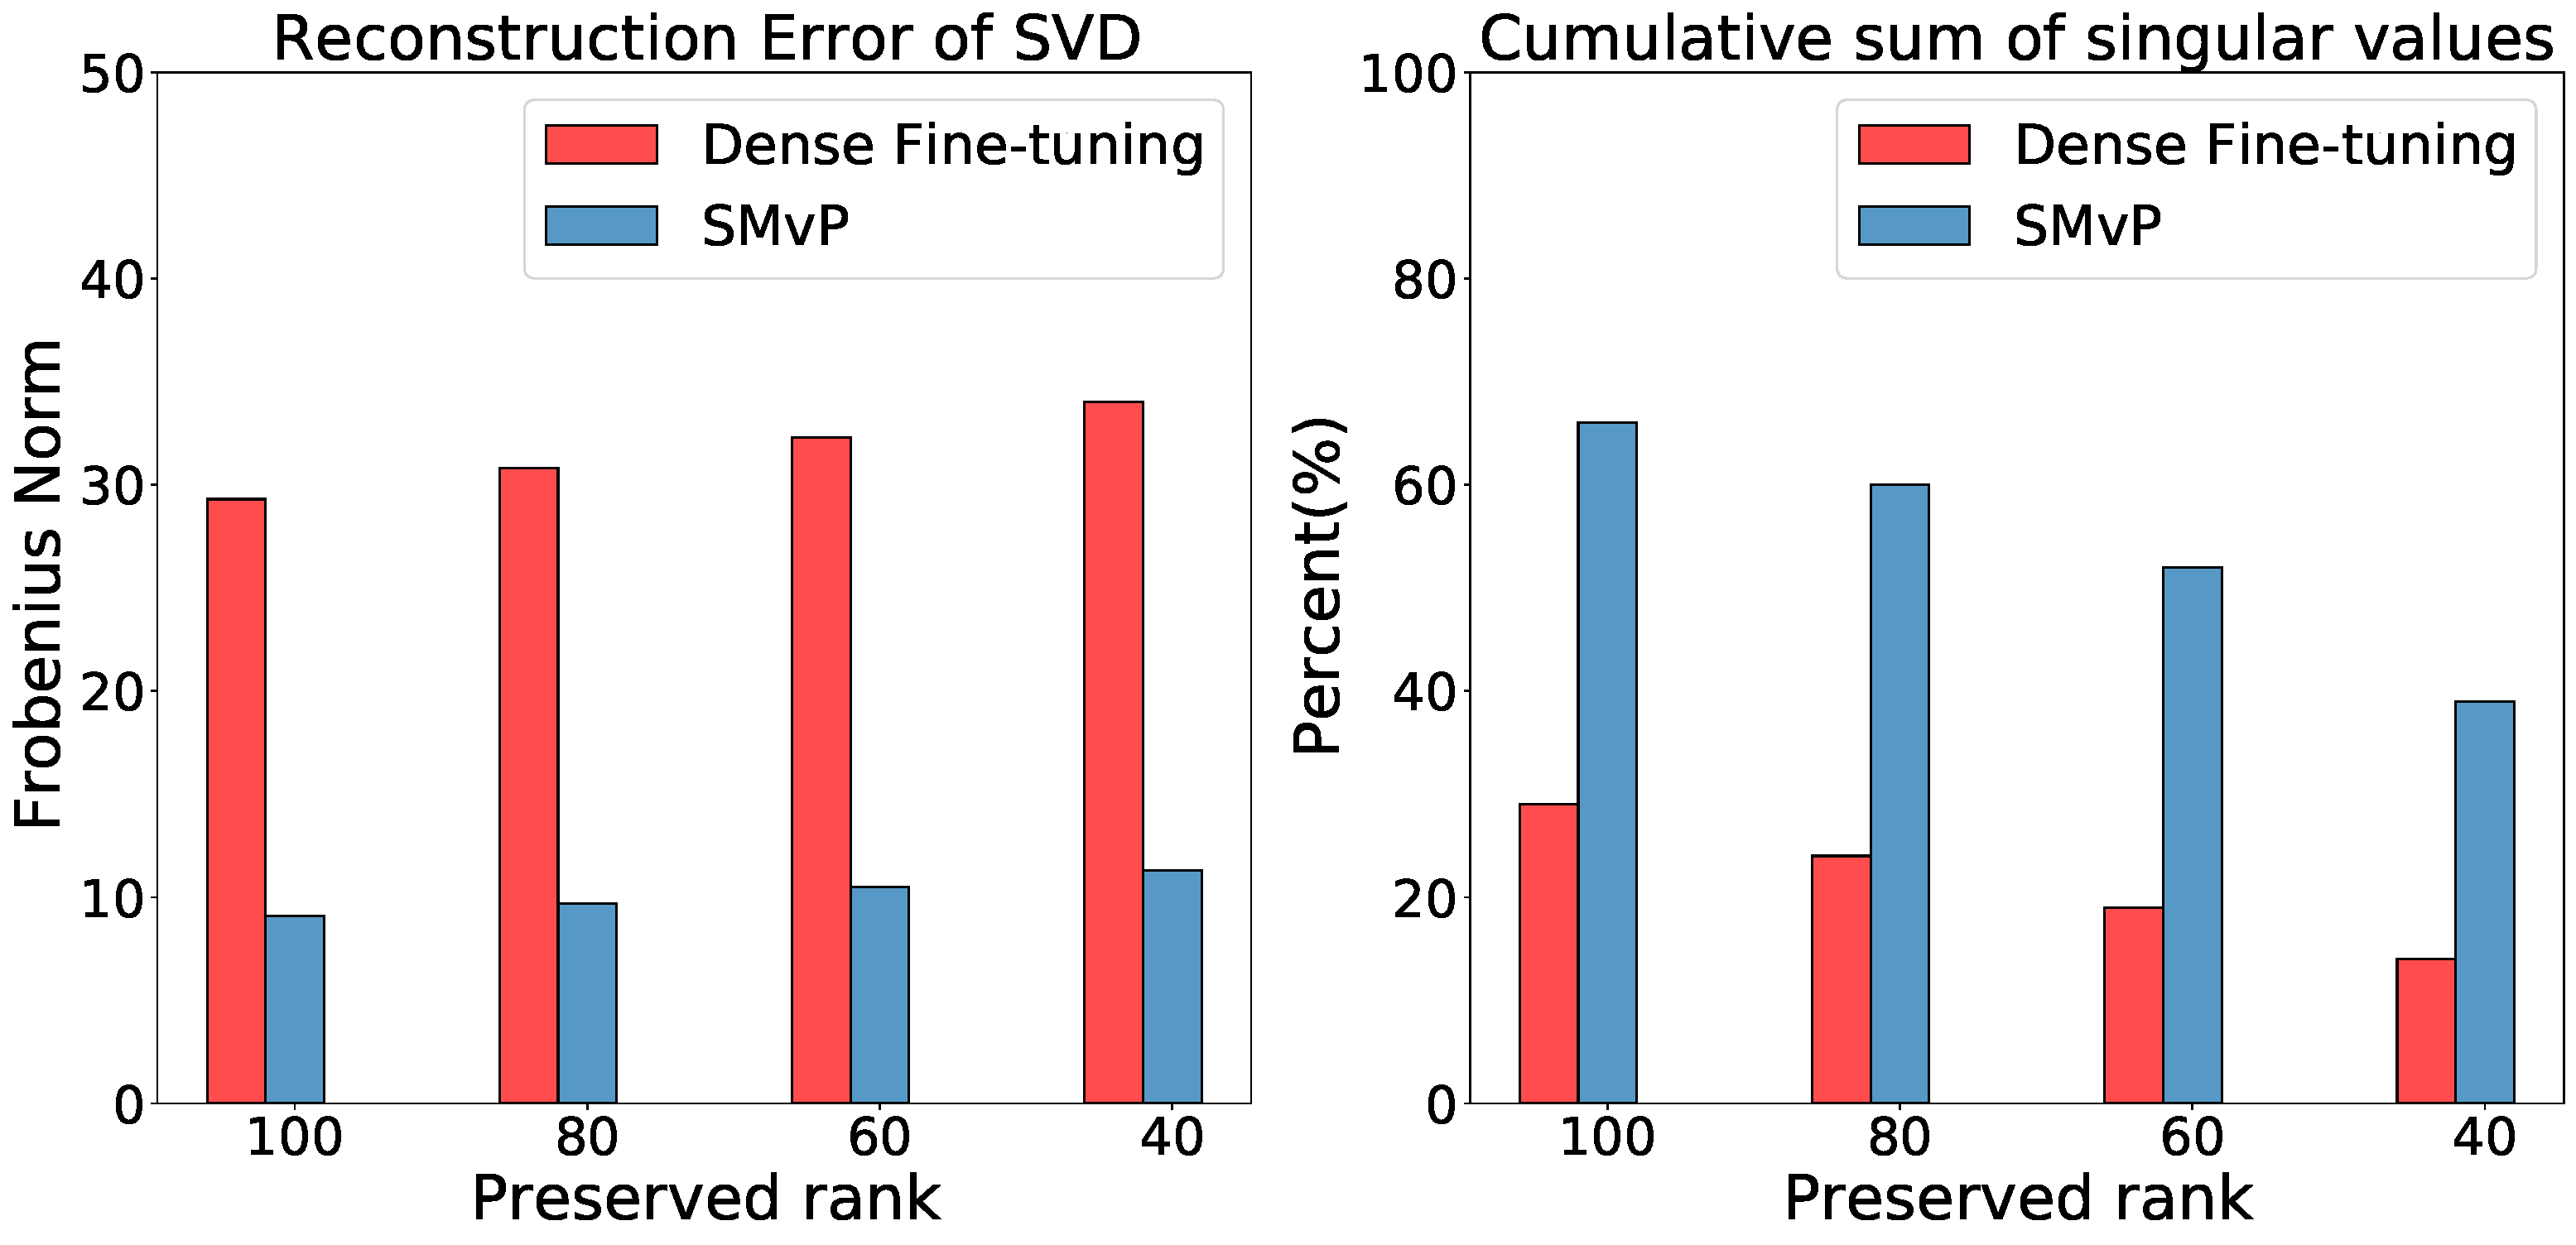
\includegraphics{./figures/norm_vis.pdf}}
	\caption{Quantitatively measuring approximation quality via reconstruction error~(left) and cumulative sum of singular values~(right) on QNLI.}
	\label{fig:norm}
\end{figure}
Given the competitive performance and low-rank structure of 
first-order pruning algorithms, 
it appears plausible to perform low-rank factorization on 
low-rank sparse models for model compression. 
As a sanity check of its feasibility, we quantitatively measure the 
quality of low-rank approximation with various preserved ranks $k$. 
\figref{fig:norm} shows that given a specific $k$, 
the sum of top-$k$ singular values of matrices produced by SMvP takes a much larger portion of total values than fine-tuning, suggesting that we can reserve more information of low-rank sparse matrix given the same $k$. The reconstruction error~(measured by Frobenius norm) of SMvP is also significantly lower, implying a higher approximation quality. We thus expect that low-rank factorization 
on low-rank sparse models to effectively combine: 
(1) the good performance of first-order pruning; 
(2) direct memory and computation reduction by 
matrix decomposition.

\section{LPAF: Low-rank Prune-And-Factorize}
\label{sec:approach}
Here we formally propose the LPAF~(\textbf{L}ow-rank \textbf{P}rune-\textbf{A}nd-\textbf{F}actorize) framework 
for language model compression. In addition, 
we propose two optimizations in the 
initialization and training of the compression process.

\subsection{The Overall Workflow}
\label{sec:ptf}
\begin{algorithm}[h]
	\caption{LPAF: Low-rank Prune-And-Factorize} %算法的名字
	\hspace*{0.02in} {\bf Input:} %算法的输入, \hspace*{0.02in}用来控制位置,同时利用 \\ 进行换行
	large pre-trained model $T$, training set $D$, first-order pruning method $P(\cdot,\cdot, \alpha)$, preserved rank $k$.\\
	\hspace*{0.02in} {\bf Output:} %算法的结果输出
	the compressed model $T_{factorized}$.
	\begin{algorithmic}[1]
		\State $T_{sparse}$ $\leftarrow$ $P(T, D, \alpha)$
		\State $T_{factorized}$ $\leftarrow$ $\text{Sparsity-aware SVD}(T_{sparse}, k)$
		\State $T_{factorized}$ $\leftarrow$ $\text{Mixed-rank Fine-tuning}(T_{factorized})$
		% \State \Return $T_{factorized}$
	\end{algorithmic}
	\label{alg:lpaf}
\end{algorithm}

%\KZ{In the overall flow, can we just simply say there are 3 steps:
%1) prune the input $T$ to a sparse matrix $T'$,
%2) factorize $T'$ into $T''$, and 3) fine-tune $T''$ according to task.
%Our first contribution, which was inspired by your prelim study, is
%this 3-step process. Our next two contributions are the optimizations on
%step 2 and 3. Isn't this clearer?}
Given a pre-trained language model $T$ and a downstream task with training set $D=\{(x_i, y_i), i=1,2,...M\}$, LPAF consists of three steps to realize model compression: 
\begin{itemize}
	\item Step-1: applying a specific first-order pruning algorithm $P(\cdot, D, \alpha)$ to obtain the task-specific low-rank sparse model $T_{sparse}=P(T,D, \alpha)$, where $\alpha$ is a hyper-parameter that controls the trade-off between performance and sparsity, e.g., $\tau$ in SMvP and CAP. 
	\item Step-2:  performing matrix factorization on each weight matrix~(excluding the embedding layer) in $T_{sparse}$ and  obtain its low-rank factorized form $T_{factorized}$. The perceivable reduction of model's memory footprint and computation cost happens at this step.
	\item Step-3:  fine-tuning $T_{factorized}$ on $D$ again using task-specific loss function until convergence. Since step 2 inevitably loses certain task-specific information, this step is designed to ensure that the compressed model retain good task performance.
\end{itemize}


%the first step of LPAF is to apply a certain first-order pruning algorithm 
%$P(\cdot, D, \alpha)$ to obtain the task-specific 
%low-rank sparse model $T_{sparse}=P(T,D, \alpha)$. 
%\KZ{We gotta be careful with our wording: is it a framework or an algorithm? If it's a framework,
%then the first step 1st-order pruning algorithm can be substituted with any other such algo and
%the framework should still work well. Does our experiment support that? If we only show the results of
%SMvP then someone may say the good results are due to SMvP and not to our framework.}
%Here 
We further present two novel optimizations, namely \textit{sparsity-aware SVD} and \textit{mixed-rank fine-tuning}, that improves the matrix factorization and fine-tuning process in step 2 and step 3 respectively. The overall workflow of LPAF with the two optimizations is shown in Algorithm \ref{alg:lpaf}.

\subsection{Optimizations}
\subsubsection{Sparsity-aware SVD}
\label{sec:sasvd}
SVD has been shown~\cite{bestsvd} to provide the optimal rank-$k$ approximation to $\bm{W}$ with respect to the Frobenius norm:
\begin{align}
	\nonumber
	\min_{\bm{A},\bm{B}} ||\bm{W}-\bm{A}\bm{B}||_{F}&=\min_{\bm{A},\bm{B}} \sum_{i,j}(\bm{W}_{i,j}-(\bm{AB})_{i,j})^2 \\
	& \text{s.t.}~~~~\text{rank}(\bm{AB})=k
\end{align}
It is a generic factorization method in that it is applicable to any matrix $\bm{W}$ by penalizing the reconstruction error of each individual weight equally. 

In our case, $\bm{W}$ is a sparse matrix from $T_{sparse}$ in which the majority of weights are set to zero by the pruning algorithm $P$. These zero weights are deemed to have less impact on the task performance compared to the retained~(unpruned) weights. However, the vanilla SVD treates each weight equally without considering the inherent sparseness of $W$, thus may be sub-optimal for preserving useful information in $W$ about the end task.
To address this issue, we propose sparsity-aware SVD which considers different priorities of parameters and weighs the individual reconstruction error based on its importance score $S_{i,j}$:
\begin{align}
	\min_{\bm{A},\bm{B}}\sum_{i,j}\bm{S}_{i,j}(\bm{W}_{i,j}-(\bm{AB})_{i,j})^2~~~\text{s.t.}~~\text{rank}(\bm{AB})=k
	\label{eq:sasvd}
\end{align}
In this way, parameters that are more important can be better reconstructed, hence retaining more task performance from $T_{sparse}$ at initialization. Nevertheless, \eqnref{eq:sasvd} does not have a closed form solution~\cite{weightedsvd,hsu2021language} when each $\bm{W}_{i,j}$ has its own weight. We therefore resort to a simplification by letting the same row of $\bm{W}$ share the same importance. The importance for row $i$ is given by $\hat{S}_{i}=\frac{\sum_{j}\bm{S}_{i,j}}{\sum_{n}\hat{S}_{n}}$. Let $\hat{\bm{I}}=diag(\hat{S}_1,\hat{S}_2,...,\hat{S}_{n})$ denote a diagonal matrix,  \eqnref{eq:sasvd} is now converted to:
\begin{align}
	\min_{\bm{A},\bm{B}}||\hat{\bm{I}}\bm{W}-\hat{\bm{I}}\bm{A}\bm{B}||_F~~~~\text{s.t.}~~\text{rank}(\bm{AB})=k
\end{align}
This essentially amounts to applying rank-$k$ SVD upon $\hat{\bm{I}}\bm{W}$, i.e., $\hat{\bm{I}}\bm{W}=\hat{\bm{U}}\hat{\bm{\Sigma}}\hat{\bm{V}}^\mathrm{T}$. Then the solution of $\bm{A}$ and $\bm{B}$ can be analytically obtained by:
\begin{align}
	\bm{A} &= \hat{\bm{I}}^{-1}\hat{\bm{U}}_{[:,:k]}\hat{\bm{\Sigma}}_{[:k,:k]},\bm{B}=\hat{\bm{V}}_{[:,:k]}^{\mathrm{T}}
\end{align}


\subsubsection{Mixed-rank Fine-tuning}
Recall that the last step of LPAF is to fine-tune $T_{factorized}$ on the training set $D$. This process has been proven essential to regain the performance lost during factorization~\cite{svd}. However, during the experiments, we observe the performance of fine-tuned $T_{factorized}$ still slightly lags behind $T_{sparse}$ given similar parameter budget. 
%\KZ{Isn't it normal for $T_{factorize}$ to lag behind $T_{sparse}$? Is there any evidence (experimental results) to show
%this ``lagging''?  Even in Fig. 3, in most cases, $T_{sparse}$ is still better Ours. 
%So I don't see enough motivation for this Mixed-rank fine-tuning.} 
We posit that, due to the reduced capacity~(less trainable parameters) and model-level approximation error incured by low-rank factorization, joint fine-tuning of low-rank matrices may converge to sub-optimal solutions with lower generalization ability. To mitigate this problem, we propose mixed-rank fine-tuning, a regularized scheme for training low-rank matrices.

Let $\{(\bm{A}\bm{B})_i, i=1,2...,N\}$ denotes all low-rank matrices in $T_{factorized}$. During training, for each $(\bm{A}\bm{B})_i$, we sample a binary Bernoulli random variable $z_i\sim \text{Bernoulli}(p)$, where $p$ is a global hyper-parameter. Then, the local computation process involving $(\bm{A}\bm{B})_i$ is modified to:
\begin{align}
	\bm{x}_{out} = (1-z_i)*(\bm{A}\bm{B})_i \bm{x}_{in} + z_i * \bm{W}_i\bm{x}_{in}
\end{align}
where $\bm{W}_i$ is the sparse matrix in $T_{sparse}$ from which $\bm{A}_i$ and $\bm{B}_i$ are derived. In this way, the low-rank matrices can further 
benefit from gradient-level regularization from  $T_{sparse}$, 
thus reducing the generalization gap. The hyper-parameter $p$ is controlled by a scheduler. We implement it such that $p$ is linearly decayed from an initial value $p_{init}$ to zero by a constant step size $d$:
\begin{align}
	p = \text{max}(0, p_{init}-d*t)
\end{align}
As $p$ decreases, $\bm{W}_i$ is gradually substituted by low-rank sub-matrices $(\bm{AB})_i$. When $p$ reaches zero, the training enters the phase of standard fine-tuning. To mitigate the instability introduced by sampling, we let each input go through the forward pass twice with different $\bm{z}^1=\{z_i^1\}_{i=1}^{N}$ and $\bm{z}^2=\{z_i^2\}_{i=1}^{N}$, and impose a consistency objective on the two outputs to promote stability:

\begin{align}
	\mathcal{L}_{c}=\mathcal{D}(y_{\bm{z}^1}, y_{\bm{z}^2})
\end{align}
where $\mathcal{D}$ can be the Kullback-Leibler divergence for classification tasks and the MSE loss for regression tasks.

% After $p$ reaches zero, the model still benefits from the regularization effect brought by different dropout masks~\cite{rdrop}.
